\section{Web Tabanlı Konteyner Orkestrasyon Sistemi}\label{sec:project}
Bu proje, kullanıcıların konteyner teknolojilerini kullanarak konteynerlerle etkileşimde bulunmasını sağlayan bir web arayüzü sağlar. Proje, kullanıcıların hazırlanan bir formu doldurarak konteyner oluşturma, çalıştırma ve konteynerden gelen çıktıları grafik ve tablo şeklinde elde etme imkanı sunar.\\
Ayrıca, projenin kullanıcı arayüzü ve arkaplan (backend) işleyişi hakkında da bilgi verilmektedir.
\subsection{Kullanıcı Arayüz}
Kullanıcı arayüzü, özel bir template seçilerek projenin gereksinimlerine uygun hale getirilmiştir. Template içerisinde gereksiz kısımlar temizlenerek sağ menü bölümü oluşturulmuştur. Bu sayede kullanıcılar, sağ menü üzerinden kolayca erişebilecekleri Dashboard, görevler (Ping, Theharvester), sistem logları ve Profil gibi önemli bölümlere ulaşabilmektedir. Bu düzenlemeler, arayüzün kullanıcı dostu ve projeye özgü bir hale gelmesini sağlamaktadır.

\textbf{Oturum Açma} : Kullanıcıların uygulamayı kullanabilmek için oturum açmalarını sağlar. Kullanıcı, kayıtlı e-posta adresi ve şifresini girerek oturum açma işlemini gerçekleştirir.
\begin{figure}[ht]
  \centering
  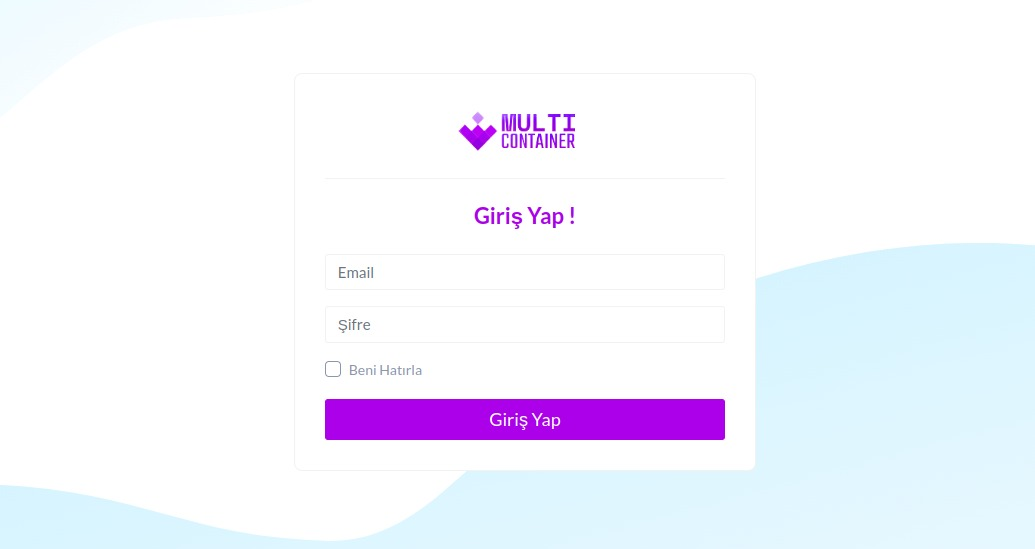
\includegraphics[width=0.6\linewidth]{images/login.jpeg}
  \caption{Giriş Sayfası}
  \label{fig:login}
\end{figure}

Şekil \ref{fig:login}'de görüldüğü gibi oturum açma sayfası, kullanıcıya e-posta ve şifre alanlarını doldurarak oturum açma imkanı sunar. Kullanıcının girdiği e-posta adresi ve şifre, kayıtlı bilgilerle doğrulandıktan sonra oturum açma işlemi tamamlanır.

Kullanıcı oturumu başarıyla açtığında, \textbf{Kontrol Paneli} sayfasıyla karşılaşacaktır. Şekil \ref{fig:dashboard}'de görüldüğü gibi, bu sayfa kullanıcıya genel bir bakış sağlar ve Ping ve Theharvester konteynerlerine ilişkin istatistikleri grafik ve tablo şeklinde sunar.

\begin{figure}[ht]
  \centering
  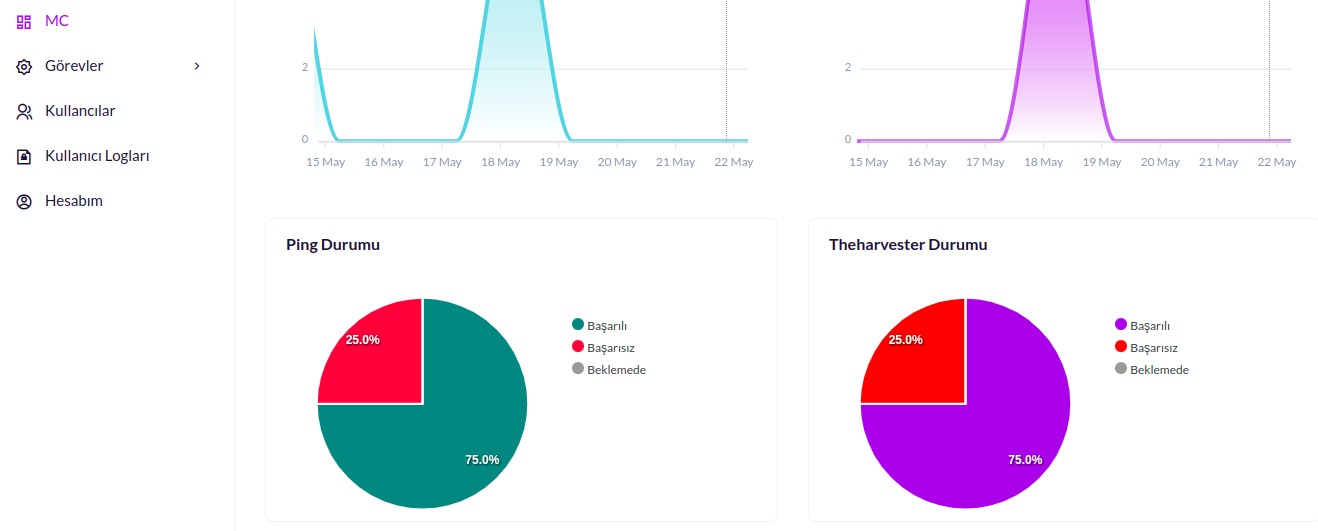
\includegraphics[width=0.6\linewidth]{images/dashboard.jpeg}
  \caption{Kontrol Paneli Sayfası}
  \label{fig:dashboard}
\end{figure}

Kontrol Paneli sayfasında kullanıcı, Ping ve Theharvester konteynerlerine ait verileri kolayca görüntüleyebilir. İlk olarak, kullanıcının sahip olduğu konteynerlerin sayısı bir grafikle gösterilir. Bu grafik, belirli bir zaman diliminde kullanıcının konteynerlerinin değişimini görsel olarak sunar.

Ardından, Ping ve Theharvester görevlerinin istatistikleri gösterilir. Kullanıcı, başarılı, başarısız ve beklemede olan görevlerin sayısını görüntüleyebilir. Bu bilgi, kullanıcının görevlerinin durumunu hızlıca anlamasına yardımcı olur.

Sayfanın alt kısmında, en son 5 görev tablo şeklinde listelenir. Bu liste, kullanıcının en son gerçekleştirdiği görevleri ve ilgili bilgileri içerir. Kullanıcılar, bu tablo üzerinden son görevlerini takip edebilir ve detaylı bilgilere erişebilir.

Kontrol Paneli sayfası, kullanıcıların konteynerlerine ilişkin genel bir bakış elde etmelerini ve önemli istatistikleri görsel ve tablo şeklinde görüntülemelerini sağlar. Bu sayede kullanıcılar, uygulamanın sağladığı konteyner orkestrasyon sisteminin performansını hızlıca değerlendirebilirler.

Panelden yeni görevler oluşturmak için \textbf{Ping Oluşturma Sayfası} kullanılır. Şekil \ref{fig:create}'de gösterilen form, kullanıcının Ping görevlerini oluşturmasını sağlar.

\begin{figure}[ht]
  \centering
  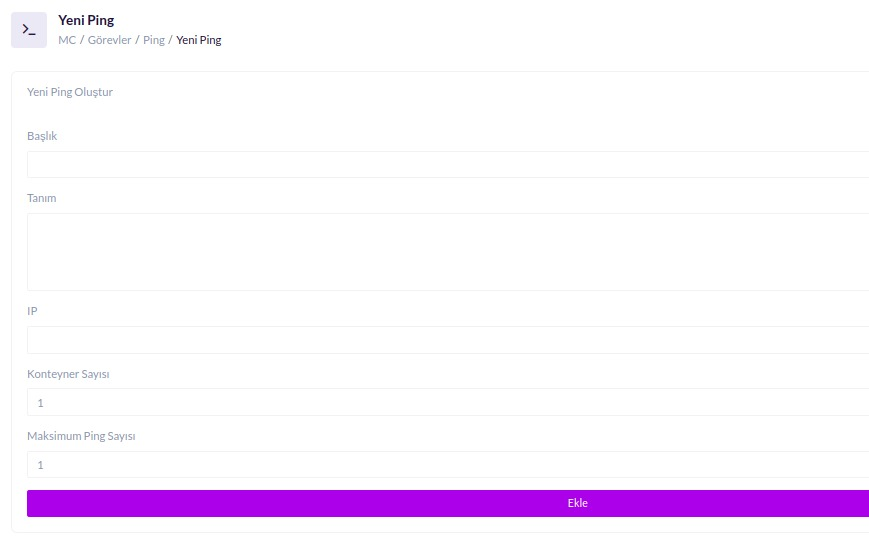
\includegraphics[width=0.6\linewidth]{images/create.jpeg}
  \caption{Ping Oluşturma Sayfası}
  \label{fig:create}
\end{figure}

Formda, kullanıcıdan aşağıdaki bilgileri girmesi istenir:
\begin{itemize}
  \item Görev Başlığı: Oluşturulacak görevin başlığı.
  \item Açıklama: Görevle ilgili detaylı açıklama.
  \item Ping IP Adresi: Ping işleminin gerçekleştirileceği hedef IP adresi.
  \item Ping Sayısı: Kaç adet ping atılacağı.
  \item Konteyner Sayısı: Bu görevi gerçekleştirecek konteynerlerin sayısı.
\end{itemize}

Bu bilgilerin tamamı zorunlu alanlardır ve kullanıcı tarafından doldurulması gerekmektedir. Kullanıcılar, bu formu doldurarak yeni Ping görevleri oluşturabilir ve bu görevlerin konteynerler tarafından gerçekleştirilmesini sağlayabilir.

Ping Oluşturma Sayfası, kullanıcılara kolay ve kullanıcı dostu bir şekilde yeni görevler oluşturma imkanı sunar. Kullanıcılar, bu form üzerinden gerekli bilgileri girerek istedikleri Ping görevini tanımlayabilir ve uygulamanın konteynerler aracılığıyla bu görevi gerçekleştirmesini sağlayabilirler.

Oluşturulan Ping görevleri, \textbf{Ping Görev Listesi} adı verilen bir tablo şeklinde görüntülenir. Şekil\ref{fig:ping_list}'de gösterilen tabloda, her görevin aşağıdaki bilgileri listelenir:

\begin{itemize}
  \item Görev Başlığı: Oluşturulan görevin başlığı.
  \item konteyner: Oluşturulan konteyner sayısı.
  \item Oluşturan: Görevin kimin tarafından oluşturuldu
  \item Durumu: Görevin mevcut durumu, başlangıçta "Beklemede" olarak gösterilir.
  \item Görev Oluşturma Tarihi
  \item Detay Botunu: Görev detayı görüntülebilmektir
\end{itemize}

\begin{figure}[ht]
  \centering
  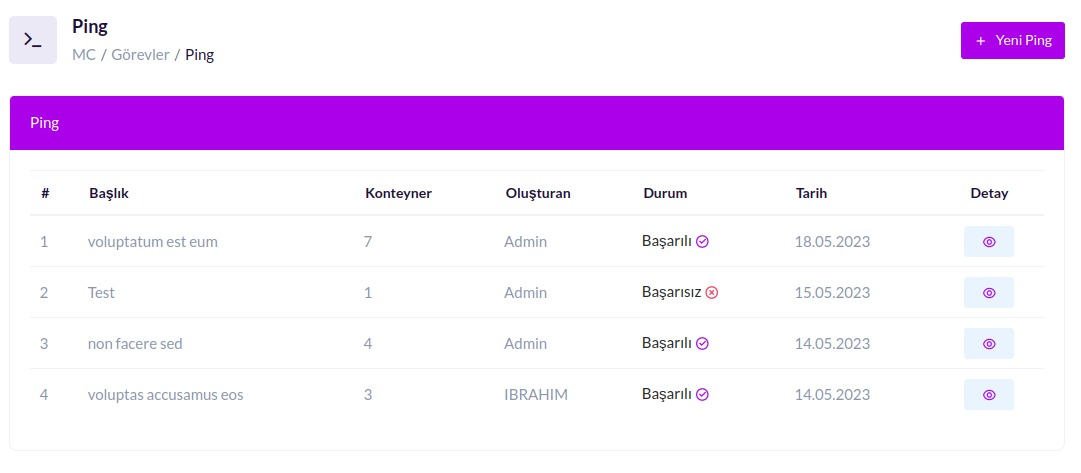
\includegraphics[width=0.6\linewidth]{images/ping_list.jpeg}
  \caption{Ping Görev Listesi}
  \label{fig:ping_list}
\end{figure}

Görevlerin işlem durumu tamamlandığında, kullanıcılar detaylarına erişebilir. Görev detayı aşağıdaki bölümlerden oluşur:
\begin{itemize}
  \item Konteyner Grafikleri: Görevin çalıştırıldığı konteyner sayısına göre grafikler oluşturulur. Her grafikte, minimum, ortalama, maksimum ping değerleri ve ping kaybı gösterilir. Şekil\ref{fig:container_graphic}'de bu grafiklerin bir örneği görülebilir.
  \begin{figure}[ht]
    \centering
    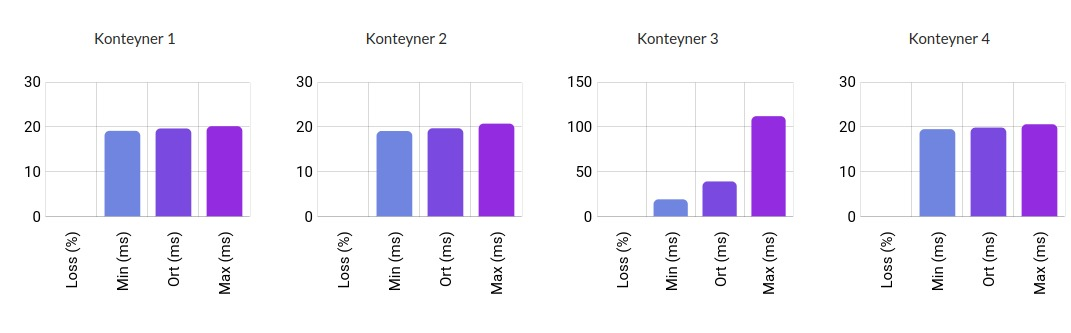
\includegraphics[width=0.6\linewidth]{images/ping_graphic.jpeg}
    \caption{konteyner Grafikleri}
    \label{fig:container_graphic}
  \end{figure}
  
  \item Görev Detayı: Görevin genel detayları, başlığı, açıklaması, atılan ping IP adresi, ping sayısı ve kullanılan konteyner sayısı gibi bilgiler içerir. Şekil\ref{fig:ping_detail}'de bu detayların bir örneği görülebilir.
  \begin{figure}[ht]
    \centering
    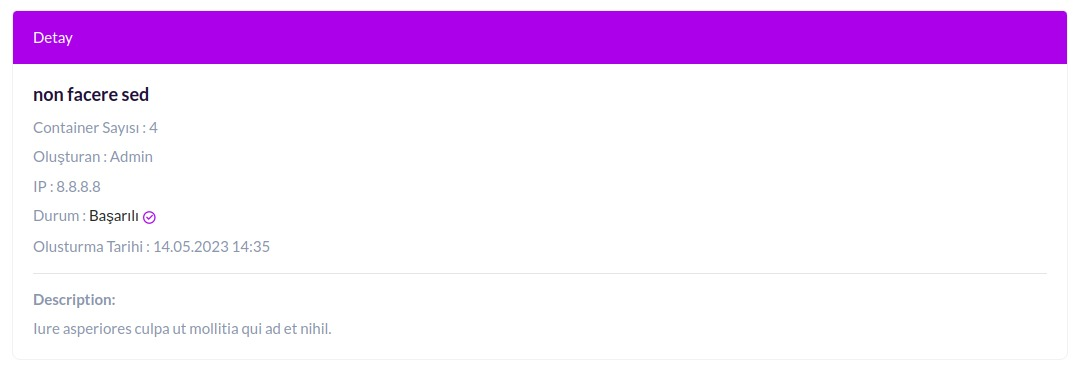
\includegraphics[width=0.6\linewidth]{images/ping_detail.jpeg}
    \caption{Ping Görev Detayi}
    \label{fig:ping_detail}
  \end{figure}
  
  \item Konteyner Detayları ve Çıktıları: Görevin çalıştırıldığı konteynerlerin ayrıntıları ve çıktıları bu bölümde görüntülenir. Konteynerlerin detaylarını içeren bir tablo ve her konteynerin çıktılarını gösteren ayrı bir tablo bulunur. \ref{fig:container_detail} ve \ref{fig:container_output} bu detayların örneklerini gösterir.
  \begin{figure}[ht]
    \centering
    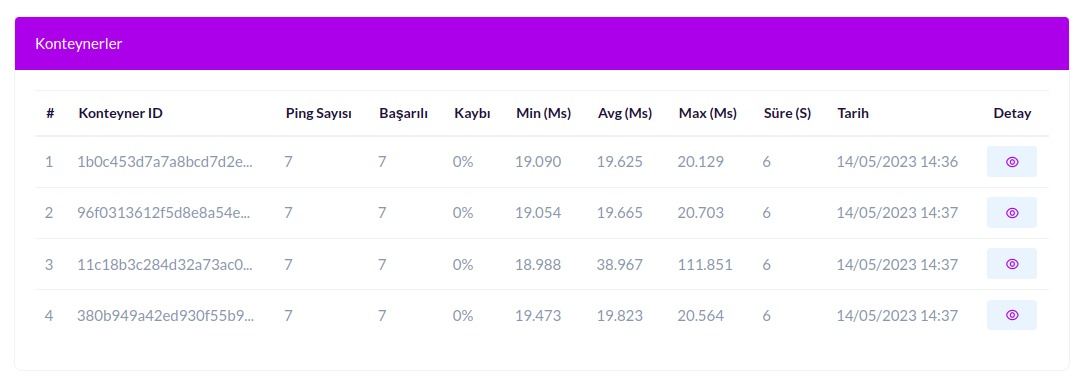
\includegraphics[width=0.6\linewidth]{images/container_detail.jpeg}
    \caption{Konteyner Detayi}
    \label{fig:container_detail}
  \end{figure}

  \begin{figure}[ht]
    \centering
    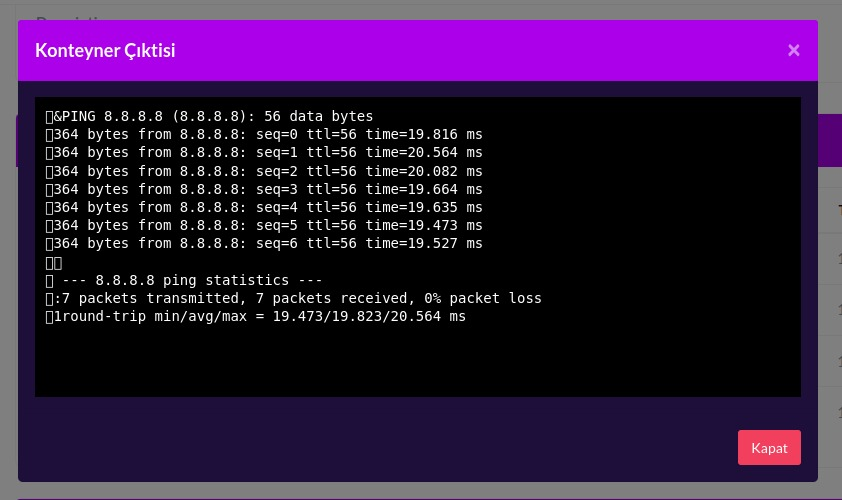
\includegraphics[width=0.6\linewidth]{images/container_output.jpeg}
    \caption{Konteyner Çıktısı}
    \label{fig:container_output}
  \end{figure}
  \item Görev sırasında oluşan hatalar bu tabloda listelenir. Her hata, hata mesajı ve hatanın oluştuğu konteyner bilgileriyle birlikte gösterilir. Şekil \ref{fig:container_error}'de bu hata listesinin bir örneği görülebilir.
  \begin{figure}[ht]
    \centering
    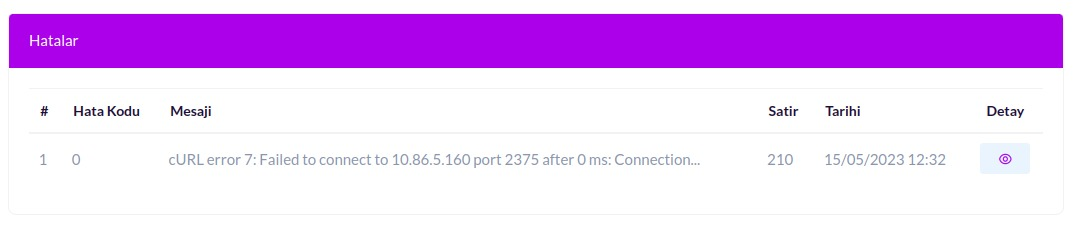
\includegraphics[width=0.6\linewidth]{images/container_error.jpeg}
    \caption{Konteyner hataları}
    \label{fig:container_error}
  \end{figure}
\end{itemize}

Bu görev detayları, kullanıcılara görevlerin ayrıntılı bilgilerini, konteyner performansını, çıktıları ve oluşan hataları inceleme imkanı sunar. Kullanıcılar, bu detaylar sayesinde görevlerin çalışma durumunu, konteynerlerin performansını ve olası sorunları kolayca analiz edebilirler.

\textbf{Kullanıcılar} bölümünde, kullanıcıların oluşturulması, görüntülenmesi, güncellenmesi ve silinmesi gibi işlemler gerçekleştirilebilir. Şekil \ref{fig:users}'de, \textbf{Kullanıcılar Listesi} adı verilen bir tablo şeklinde kullanıcıların listelendiği görülmektedir.

Her kullanıcı için aşağıdaki bilgiler listelenir:
\begin{itemize}
  \item Kullanıcı Adı ve Soyadı.
  \item E-posta: Kullanıcının kayıtlı e-posta adresi.
  \item Oluşturma Tarihi: Kullanıcının oluşturulma tarihi.
  \item İşlem sütünüde mevcuttur.
\end{itemize}

Bu tablo, sisteme kayıtlı olan tüm kullanıcıların genel bilgilerini görüntüler. Kullanıcılar, bu tablo üzerinden kullanıcıları inceleyebilir, güncelleyebilir veya silme işlemleri gerçekleştirebilir. Bu sayede sistem yöneticileri, kullanıcılarla ilgili işlemleri kolaylıkla yapabilir ve kullanıcı verilerini yönetebilir.
\begin{figure}[ht]
  \centering
  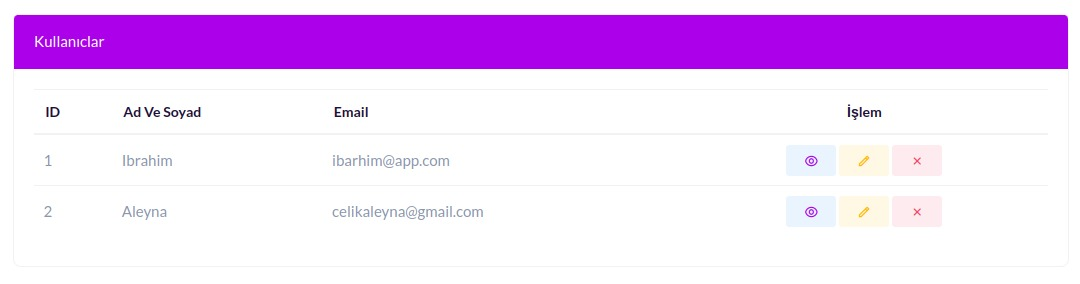
\includegraphics[width=0.6\linewidth]{images/users.jpeg}
  \caption{Kullanıcılar listesi}
  \label{fig:users}
\end{figure}

\textbf{Kullanıcı Logları} bölümünde, her kullanıcının yaptığı aktivitelerin bir log listesi olarak görüntülendiği bir tablo bulunmaktadır. Şekil \ref{fig:log}'de, Kullanıcı Logları tablosu örneği gösterilmektedir.
Bu tabloda her log girdisi için aşağıdaki bilgiler listelenir:
\begin{itemize}
  \item Kullanıcı: İlgili kullanıcının adı ve Soyadı.
  \item IP: Kullanıcının oturum açtığı IP adresi.
  \item İşlem: Kullanıcının gerçekleştirdiği işlem veya aktivite açıklaması.
  \item Tarih: İşlemin gerçekleştiği tarih.
  \item Saat: İşlemin gerçekleştiği saat.
\end{itemize}

\begin{figure}[ht]
  \centering
  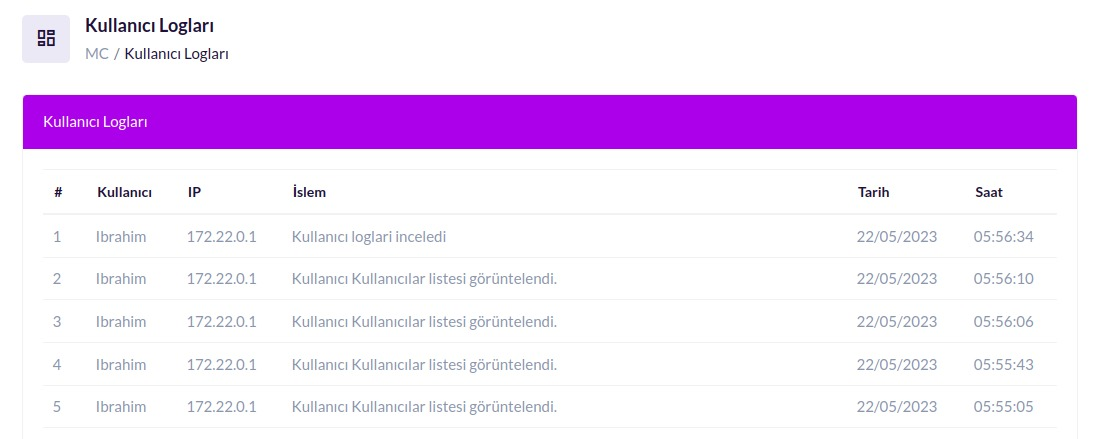
\includegraphics[width=0.6\linewidth]{images/log.jpeg}
  \caption{Kullanıcı Logları}
  \label{fig:log}
\end{figure}

Bu loglar, kullanıcı aktivitelerinin izlenmesi, takibi ve güvenlik amaçlı olarak kullanılabilir. Sistem yöneticileri veya yetkilileri, bu logları kullanarak kullanıcıların yaptığı işlemleri inceleyebilir ve gerekirse uygun önlemleri alabilir. Ayrıca, kullanıcı logları, sistemdeki kullanıcı etkinliği hakkında bilgi sahibi olmak için kullanılabilir.
\textbf{Hesabım} bölümünde, oturum açmış olan kullanıcının kendi hesap bilgilerini güncelleyebileceği bir form bulunmaktadır. Şekil \ref{fig:account}'de, "Kullanıcı Hesabım" formu örneği gösterilmektedir.
\begin{figure}[ht]
  \centering
  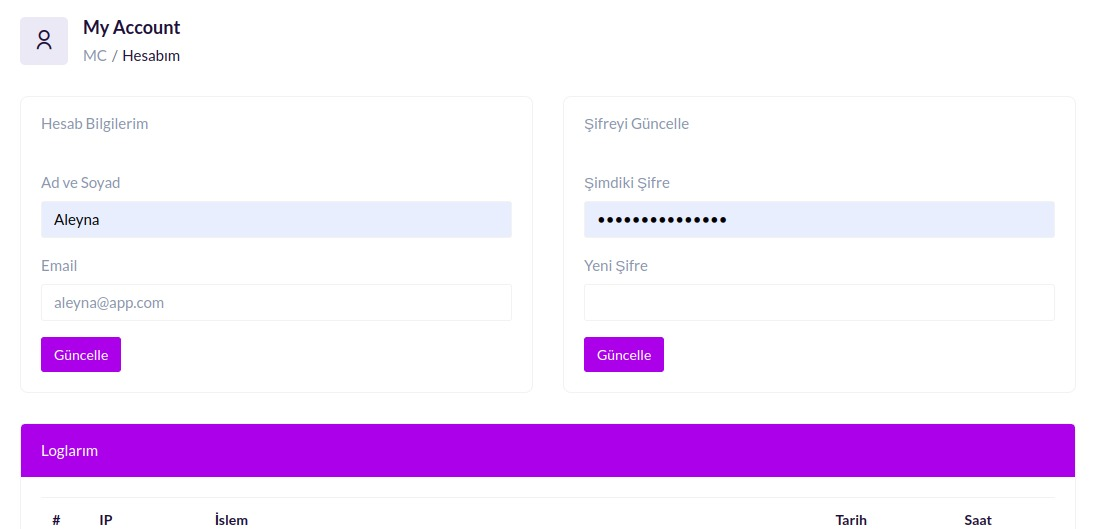
\includegraphics[width=0.6\linewidth]{images/account.jpeg}
  \caption{Kullanıcı Hesabımi}
  \label{fig:account}
\end{figure}

Ayrıca, kullanıcının kendi logları da tablo şeklinde görüntülenmektedir. Bu loglar, kullanıcının kendi aktivitelerini takip etmek ve geçmiş işlemlerini gözden geçirmek için kullanılabilir.

\subsection{Arakaplanda Çalışan Servisler (Backend)}
Bu çalışmada asıl amacı konteynerler kullanarak toplu iş yaptırmaktadır. Konteyner ne olduğunu aşağıdaki kismi anlatılmıştır.

subsubsection{Konteyner ile ilgili Temel bilgiler}
\subsection{Giriş}
Projemizin amacı, Docker kullanarak paralel işlem yapabilen sistemler, uygulamalar ve servisler için çoklu konteynerlar kullanarak bir sistem tasarlamaktır. Docker, izolasyon sağlayarak her bir konteyneri farklı özellikler ve işlevler için optimize etme imkanı sunar ve bu da uygulamanın ölçeklenebilir olmasını sağlar.
\subsection{Yapı ve Teknolojiler}
Projede, Laravel yapısı kullanıldı. Bu sayede, arayüz ve backend arasında esneklik sağlayarak birlikte çalışma imkanı elde edildi. Arayüz için başlangıçta bir hazır template kullanıldı, ancak bu templateleri ihtiyaçlarımıza göre özelleştirildi ve değişiklikler yapıldı. Daha sonra backend ile entegrasyonu gerçekleştirerek ayarlamaları tamamlandı.
\subsection{Güvenlik Önlemleri:}
Projenin güvenliği için, login sayfası tasarlandı ve erişim kısıtlamaları eklendi. Bu sayede, giriş yapmayan kullanıcıların diğer sayfalara erişmesi engellendi. Kullanıcıların güvenliğini ve verilerin gizliliğini korumak önemli bir hedefimiz oldu.
\subsection{Docker ile Konteynerleme}
Son aşamada, Docker işlemlerini gerçekleştirerek konteynerleme işlemleri tamamlandı. Docker'ın avantajlarından yararlanarak, uygulamayı farklı konteynerlar içinde çalıştırılabildi. Böylelikle, her bir konteynerin optimize edilmiş bir şekilde çalışmasını sağlayarak işleri belirtilen sayıda konteynera bölerek daha esnek bir yapı oluşturuldu. Bu da performansı artırırken sistem üzerindeki yükü dengelememize yardımcı oldu.
\subsection{İlerleme Takibi ve İletişim Sistemi}
Projenin arayüzünde, canlı olarak ilerleme bilgilerini gösteren bir özellik bulunmaktadır. Kullanıcılara, toplam iş miktarı, tamamlanma yüzdesi ve en hızlı çalışan konteynerlar gibi önemli bilgiler sunarak işlerin durumunu takip etmeleri sağlandı. Bu sayede kullanıcılar, işlerin ne kadar ilerlediğini ve hangi konteynerların en etkili olduğunu görebilmektedir.


\section{PROJE'NİN İŞLEYİŞİ}
\subsection{Arayüz Kısmı }
\subsubsection{Template Hazırlığı}
Proje için uygun bir template seçilmiş ve projenin gereksinimlerine uygun hale getirilmiştir. Template içerisinde yer alan gereksiz kısımlar temizlenerek sağ menü bölümü oluşturulmuştur. Bu sayede kullanıcılar, sağ menü üzerinden kolayca erişebilecekleri Dashboard, görevler (Ping, Theharvester), sistem logları ve Profil gibi önemli bölümlere ulaşabileceklerdir. Bu düzenlemeler, arayüzün daha kullanıcı dostu ve projeye özgü hale getirilmesini sağlamaktadır.
\subsubsection{Kullanıcı Girişi}
Projeyi ilk açtığınızda, kullanıcı login sayfasıyla karşılaşacaksınız. Bu sayfada kimlik bilgilerinizi girdikten sonra doğrulama işlemi gerçekleştirilir ve başarılı bir şekilde doğrulandığınızda diğer sayfalara erişim sağlanır. Bu sayede projenin güvenliği ve kullanıcı gizliliği sağlanırken, yetkilendirme mekanizması sayesinde sadece yetkili kullanıcılar projenin içeriğine erişebilir. Bu işlem, kullanıcıların projenin sunduğu özelliklere erişebilmeleri ve projeyi kullanmaya başlayabilmeleri için önemli bir adımdır.
\subsubsection{Kontrol Paneli}

Giriş yaptıktan sonra karşılaşacağınız ilk sayfa Kontrol Paneli olacaktır. Kontrol paneli, kullanıcılara projede gerçekleştirilebilecek işlemleri açıklayan ve sunan bir sayfadır. Bu sayede kullanıcılar, projenin farklı özelliklerini keşfedebilir, verileri yönetebilir, raporları görüntüleyebilir veya diğer kullanıcılarla etkileşimde bulunabilir. Kontrol paneli, projenin merkezi bir noktasıdır ve kullanıcılara projenin sunmuş olduğu işlevselliği keşfetme ve kullanma imkanı sağlar. Bu sayede kullanıcılar projenin potansiyelini tam olarak kullanabilir ve projenin amaçlarına yönelik işlemleri gerçekleştirebilirler.
\subsubsection{Görevler Bölümü}
Sağ menüde bulunan Görevler bölümünden, kullanıcılar yeni görevler oluşturabilir ve önceden oluşturulmuş görevlere erişebilirler. Görevler bölümü, kullanıcılara farklı işlemleri gerçekleştirmek için bir arayüz sağlar. Örneğin, bir Ping görevi oluşturulduğunda, kullanıcılar konteynırların çıktılarına, kayıp yüzdesine, maksimum, minimum ve ortalama geri dönüş sürelerine erişebilirler. Bu bilgiler, görevin durumu ve performansı hakkında önemli bilgiler sunar. Kullanıcılar, görevlerin sonuçlarını inceleyebilir, performans analizleri yapabilir ve gerektiğinde görevleri düzenleyebilirler. Görevler bölümü, kullanıcıların projede yapılan işlemleri izleme ve yönetme sürecine katkı sağlar, verimliliği artırır ve kullanıcılara kontrol sağlar.
\subsubsection{Sistem Logları}
Sağ menüde bulunan Sistem Logları bölümü, kullanıcılara log kayıtlarını görüntüleme imkanı sunar. Bu log kayıtları, kullanıcının hangi görevleri ne zaman çalıştırdığını, görevlerin tamamlanma sürelerini, başarı durumunu ve oturum açma/kapatma bilgilerini içerir. Sistem Logları bölümü, kullanıcılara gerçek zamanlı olarak yapılan işlemleri takip etme ve denetleme yeteneği sağlar. Bu sayede kullanıcılar, projenin geçmişinde gerçekleşen işlemleri izleyebilir, performans analizleri yapabilir ve gerektiğinde sorun giderme yapabilir. Sistem Logları bölümü, kullanıcılara projenin izlenebilirliğini artırırken, işlemlerin güvenliğini ve bütünlüğünü de sağlar.
\subsubsection{Hesabım Bölümü}
Hesabım bölümü, kullanıcılara profil düzenlemelerini gerçekleştirme imkanı sunar. Bu bölümde kullanıcılar, profil bilgilerini güncelleyebilir, şifrelerini değiştirebilir, iletişim tercihlerini yönetebilir ve gizlilik ayarlarını düzenleyebilir. Profil düzenlemeleri sayesinde kullanıcılar, kendi hesaplarını kişiselleştirme ve özelleştirme imkanına sahip olurlar. Bu şekilde, kullanıcılar projedeki profil bilgilerini istedikleri şekilde yönetebilir ve hesaplarını kendi ihtiyaçlarına göre ayarlayabilirler. Hesabım bölümü, kullanıcılara projedeki kişisel bilgilerini güncelleme ve yönetme kolaylığı sağlar, böylece kullanıcılar projede daha iyi bir kullanıcı deneyimi yaşayabilirler.

%arayüz fotoğrafları eklenecek 
\subsection{Arka plan işleyişi}
Projenin alt yapısı, PHP framework'ü olan Laravel kullanılarak geliştirilmiştir. Projenin çalışması için bir docker-compose.yml dosyası kullanılarak Docker'da bir servis oluşturulmuştur. Bu servis, iki konteyner oluşturarak projenin çalışmasını sağlamaktadır. Docker yönetimi için Docker Engine API kullanılmıştır.

\subsubsection{Docker Engine API}

Docker, Docker Engine API olarak adlandırılan arka plan programı sayesinde etkileşim için bir API sağlamaktadır. Docker Engine API, birçok modern programlama dilinde yer alan HTTP kütüphanesi tarafından erişilen bir RESTful API'dir. Projedeki PHP SDK güncel olmadığı için, Docker API'yi kullanarak Laravel uygulaması ile haberleşme sağlayan DockerService adında bir servis yazılmıştır. Bu sayede konteyner oluşturma, çalıştırma, detaylarını görüntüleme gibi işlemler yapılabilmektedir.

\subsubsection{Laravel Özellikleri}

Bu projede, Laravel'in sağladığı özellikler kullanılarak geliştirme yapılmıştır. Bir IP'ye ping atma görevi oluşturma süreci şu şekildedir:

Kullanıcı, ping oluşturma görevi formunu doldurmalıdır. Formda, görev başlığı, görev açıklaması, atılacak IP adresi, oluşturulacak konteyner sayısı ve her bir konteynerda kaç adet ping atılacağı gibi fieldler bulunmaktadır.

Form doldurulduktan sonra, PingRequest sınıfı devreye girecektir. Bu, Laravel'in sağladığı bir özellik olan Request'tir ve formdan gelen bilgilerin doğruluğunu sağlamaktadır. Eğer bilgiler doğruysa, PingController'a geçilir. Eğer bilgiler doğrulanamazsa, form sayfasına geri yönlendirilir ve eksik olan fieldlerin altında bir hata mesajı yazılır.

PingController, yeni bir görev oluşturarak kullanıcıyı görev listesi sayfasına yönlendirir ve "oluşturuldu" mesajını yazdırır.

Yeni bir görev oluşturulduğunda, Laravel'in bir diğer özelliği olan "Event (Tetikleyici) \& Listener (Dinleyici)" devreye girer.

Event \& Listener: Bu proje, yeni bir görev oluşturulduğunda event tetiklenir ve Listener çalışmaya başlar. Listener aracılığıyla DockerService çalıştırılır. Kullanıcıyı Form sayfasında bekletmemek için Listener kuyruğa alınır ve DockerService işlemi tamamlandıktan sonra görev durumu güncellenir. Başarılıysa 1, başarısızsa 2 olarak bildirilir
%ibrahim bu kısımda özet yazacak detaylandırılacak
 \subsection {Veritabanı kısmı İçin }
 MySQL veritabanı kullanılarak bir proje için optimize edilmiş bir veritabanı şeması oluşturuldu. Bu şema, "users" (kullanıcılar), "ping" (ping kayıtları) ve "pingcontainers" (ping konteynerleri) adında üç tabloyu içermektedir. Bu düzenleme, veritabanının performansını artırmak ve veri bütünlüğünü sağlamak amacıyla yapılmıştır.\\
"users" tablosu, kullanıcıların temel bilgilerini içerir ve her kullanıcıya birincil anahtar (ID) ile benzersiz bir kimlik atar. Ayrıca kullanıcı adı, e-posta adresi ve diğer ilgili bilgiler gibi sütunlar da içerir.\\
"pingcontainers" tablosu, kullanıcıların oluşturabileceği ping konteynerlerini temsil eder. Her konteyner birincil anahtar ile tanımlanır ve kullanıcıya ait olacak şekilde kullanıcı kimliği (user ID) ile ilişkilendirilir. Bu tablo, kullanıcının birden fazla konteyner oluşturabilmesine olanak sağlar.\\
"ping" tablosu, gerçekleşen ping olaylarını kaydetmek için kullanılır. Her ping kaydı, birincil anahtar ile tanımlanır ve bir konteynere (container ID) ve kullanıcıya (user ID) bağlanır. Bu ilişki, her ping kaydının hangi kullanıcı ve konteyner tarafından oluşturulduğunu gösterir.\\
Bu veritabanı şeması, kullanıcıların birden fazla konteyner ve görev oluşturabilmesini sağlar. Ayrıca, her görevin bir kullanıcı tarafından oluşturulduğu ilişkisi sayesinde veri bütünlüğünü korur.\\
Bu düzenleme, veritabanının daha etkili bir şekilde veri saklamasını ve verilere hızlı erişim sağlamasını amaçlamaktadır. Ayrıca, veri bütünlüğünü korumak için gereken ilişkileri de sağlamaktadır.\\
 \begin{figure}[]
    \centering
    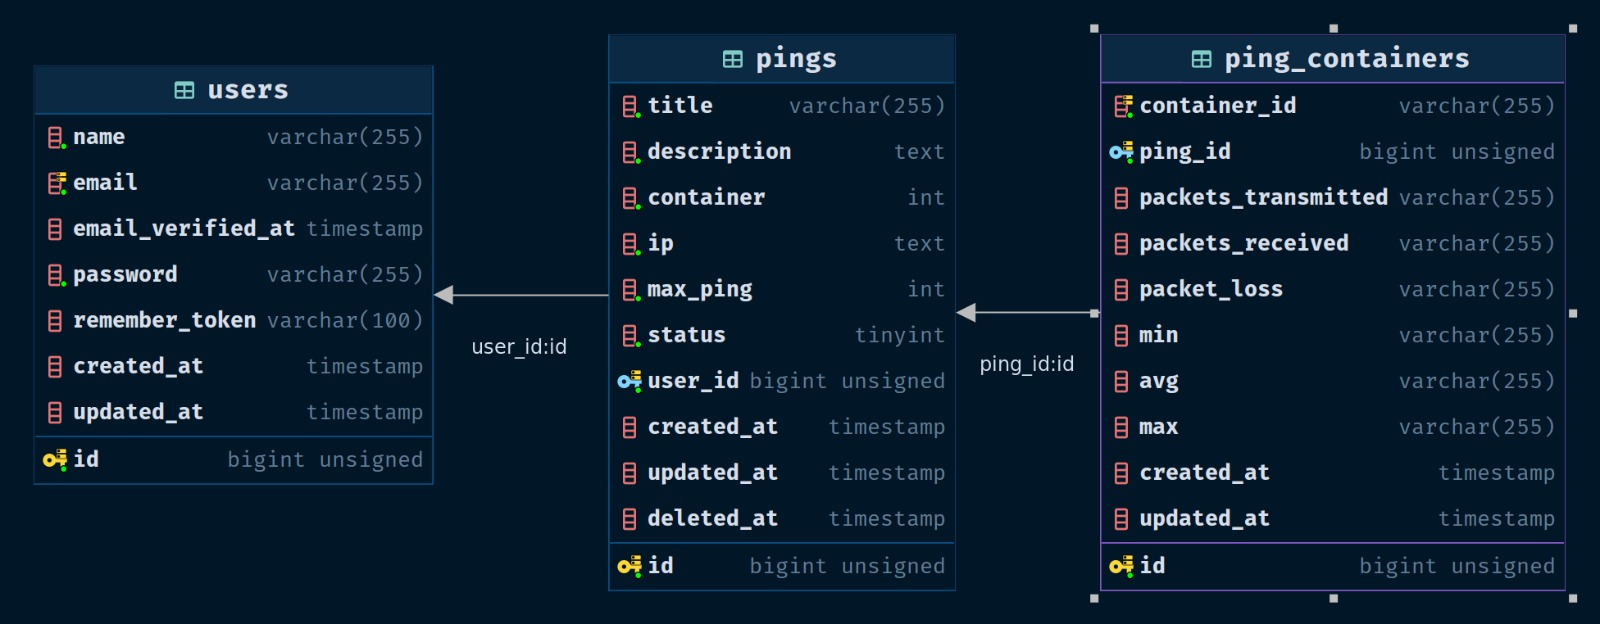
\includegraphics[width=0.9\textwidth]{images/sql.jpg}
    \caption{Sql ping tabloları}
    \label{fig:resim_etiketi}
  \end{figure}



